\vspace{-2pt}
\subsection{Evaluating Aggregation Alternatives}
\label{subsec:res-agg}



\begin{figure}[h]
\vspace{-10pt}
	\centering
		\subfloat[\#ACCs=6]{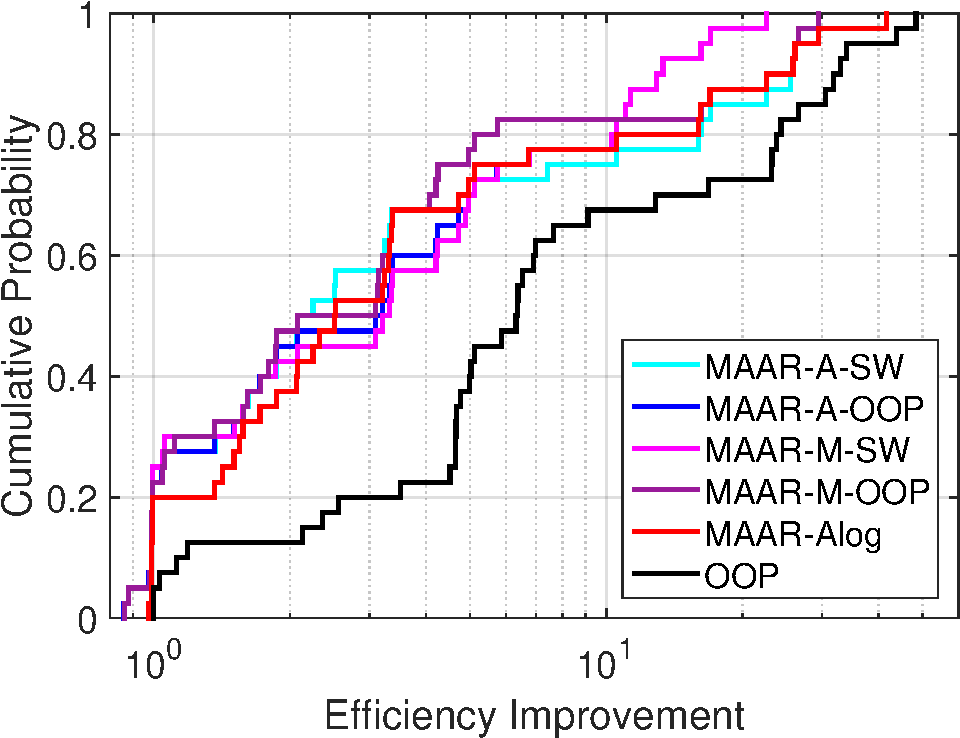
\includegraphics[width=.33\linewidth]{fig/MAARsw6.pdf}\label{fig:sw6}}
		\hfill
		\subfloat[\#ACCs=12]{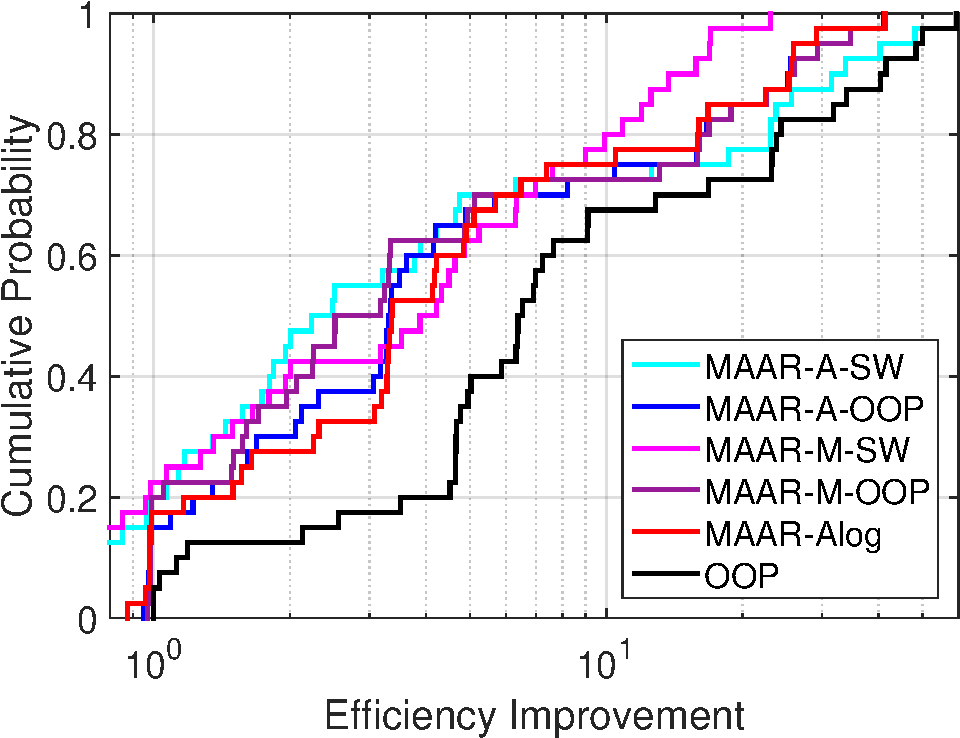
\includegraphics[width=.33\linewidth]{fig/MAARsw12.pdf}\label{fig:sw12}}
        \hfill
		\subfloat[\#ACCs=19]{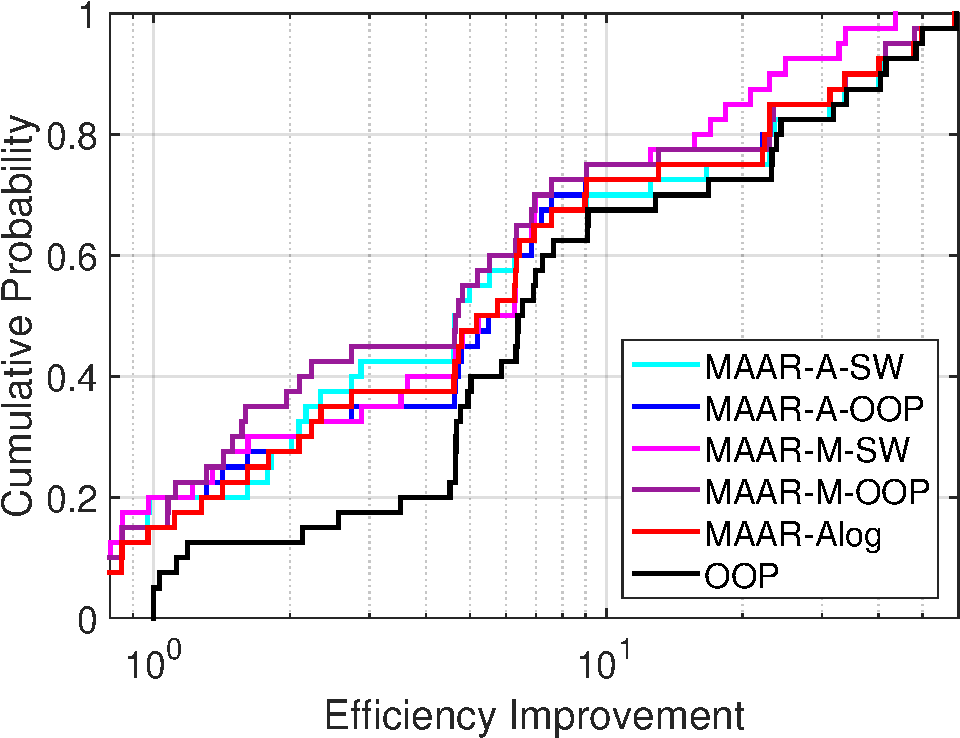
\includegraphics[width=.33\linewidth]{fig/MAARsw19.pdf}\label{fig:sw19}}
\vspace{-8pt}
	\caption{Relative Efficiency Compared with SW}
	\label{fig:OpenVXsw}
%		\vspace{-0pt}
\end{figure}



%\begin{figure}[h]
%\vspace{-10pt}
%	\centering
%		\subfloat[\#ACCs=6]{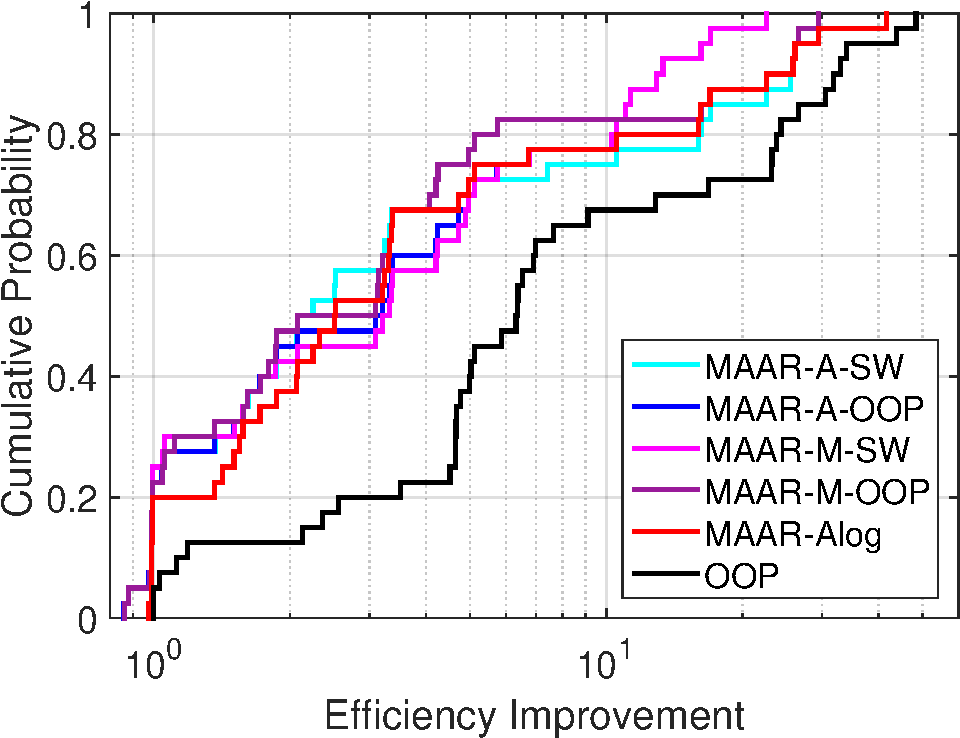
\includegraphics[width=.48\linewidth]{fig/MAARsw6.pdf}\label{fig:sw6}}
%		\hfill
%		\subfloat[\#ACCs=12]{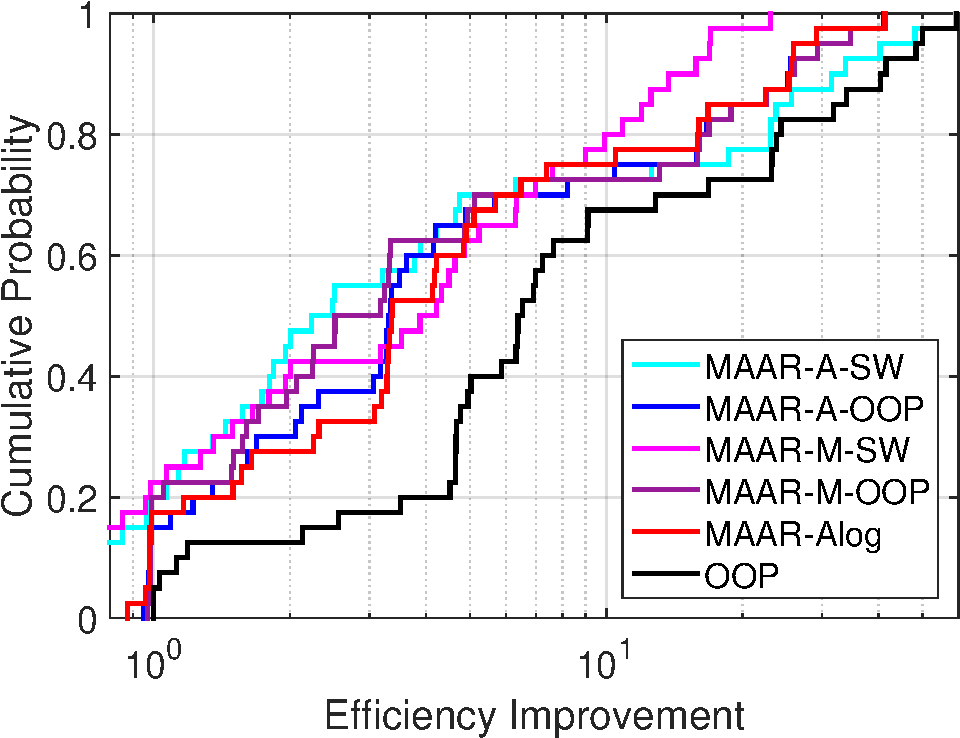
\includegraphics[width=.48\linewidth]{fig/MAARsw12.pdf}\label{fig:sw12}}
%		\\
%		\vspace{-8pt}
%		\subfloat[\#ACCs=19]{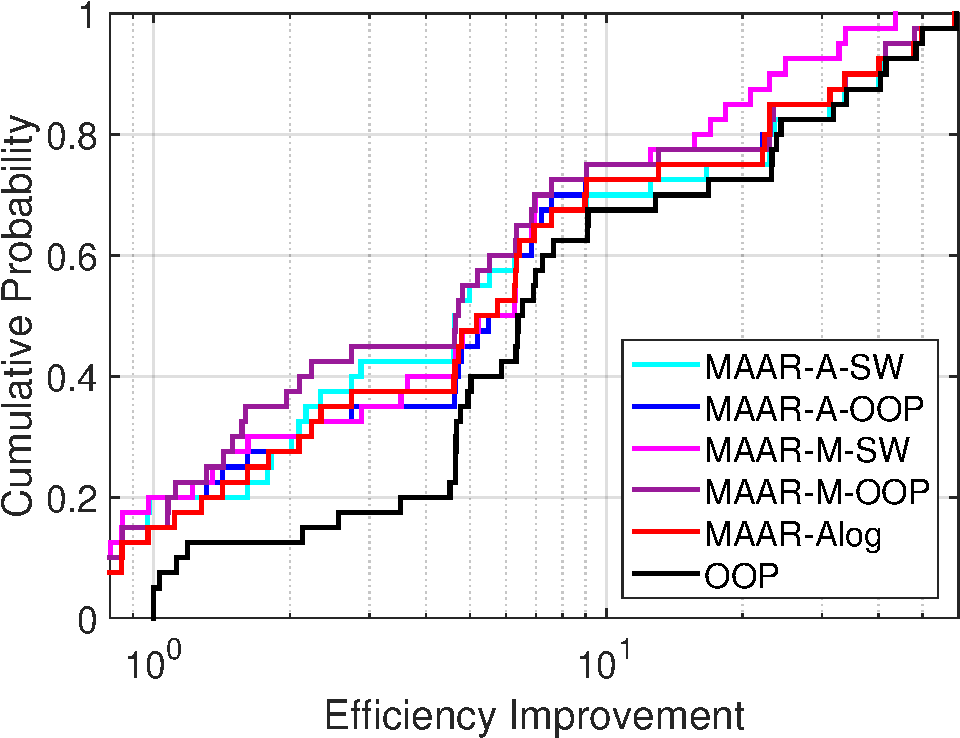
\includegraphics[width=.48\linewidth]{fig/MAARsw19.pdf}\label{fig:sw19}}
%		\hfill
%		\subfloat[\#ACCs=12]{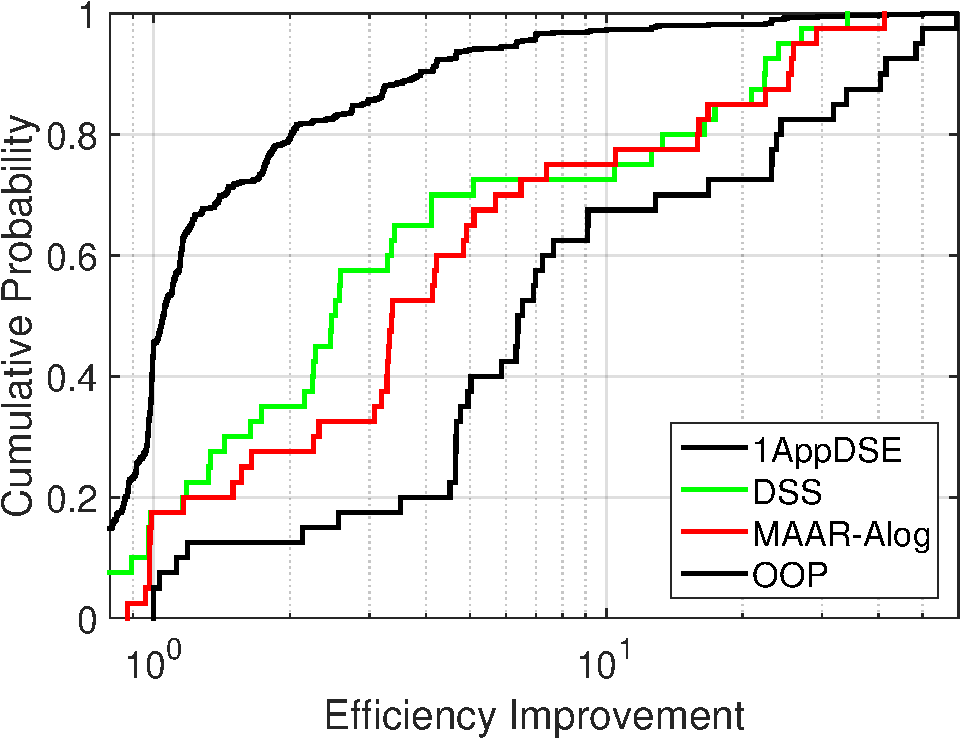
\includegraphics[width=.48\linewidth]{fig/MAARsw12all.pdf}\label{fig:sw12all}}
%		\vspace{-8pt}
%	\caption{Cumulative Relative Efficiency Compared with SW}
%	\label{fig:OpenVXsw}
%		\vspace{-0pt}
%\end{figure}

%This section discusses the impact of aggregation on the fairness when allocating a common platform.
To visualize fairness, \figref{fig:OpenVXsw} shows the cumulative probability of efficiency improvement for OOP and MAAR DSE with different aggregations given a budget (ACCs = 6, 12, 19).
The x-axis denotes efficiency improvement ($rEFF_{SW}$), and y-axis is the cumulative probability.
A point ($x$, $y$) indicates that a proportion $y$ of applications have a relative efficiency $x$ or less.  

%(so 1 - y\% have a relative efficiency of at least x).
E.g., in \ref{fig:sw6}, there is 67.5\% (0.675 in y-axis) probability that OOP has 10x ($10^1$ in x-axis) or 10x less efficiency improvement. In another description, OOP has 32.5\% ($1-0.675$ in y-axis) to achieve 10x or 10x more efficiency improvement. The line positioned more toward the bottom right has a better efficiency improvement, and OOP black line is the upper bound. With ACCs increasing from 6 (\figref{fig:sw6}) to 19 (\figref{fig:sw19}), the MAAR line moves close to OOP line, which means the efficiency improvement of MAAR platform are catching up to OOP performance. After ACCs>10, OOP has already allocated enough ACCs in each application-specific platform, and there are no remaining kernels to accelerate. In \figref{fig:OpenVXsw}, the up right parts of the lines represent high-efficiency applications, and the bottom left parts of lines show the effect of low-efficiency applications. 


%OOP lines are different between ACCs=6 and ACCs=12, but are identical between ACCs=12 and ACCs=19. The reason is that after ACCs>10, OOP has already allocated enough ACCs in each application-specific platform, and there are no remaining kernels to accelerate.


% The lines in these figures are similar to \figref{fig:effSW}, and represent efficiency improvement of each application. The difference between two types of figure is that \figref{fig:OpenVXsw} sorts the efficiency improvements for each DSE method independently and replace the applications with probability. As a result, each row in \figref{fig:effSW} represents the efficiency improvement of different methods for the same application, while \figref{fig:OpenVXsw} row may represent different applications. Then, 

Comparing among different MAAR aggregation methods, 
$A\mhyphen SW$ is good for high-efficiency applications (top 25\%), however, has an efficiency loss for other applications, especially in \figref{fig:sw12}.
$A\mhyphen OOP$ has good efficiency improvement for all applications in all HW budgets.
$M\mhyphen SW$ only achieves good performance near the median-efficiency application, and there is a significant efficiency loss for all high-efficiency applications. 
$M\mhyphen OOP$ is bad in efficiency improvement view, and it loses in both median- and low-efficiency applications. 
$M\mhyphen SW$ and $M\mhyphen OOP$ shows the median $rEFF_{SW}$ and $rEFF_{OOP}$ aggregations of the same application set are actually different. 
$Alog$ achieves good efficiency improvement for all applications, with more focusing on low-efficiency applications, compared with another good evaluation $A\mhyphen OOP$.